\model{Playing Cards}

Now let's play a different game.
In this section, we'll create an array of face cards.
(Note: The array is one-dimensional, but the cards are displayed on four lines for convenience.)

\begin{center}
% http://www.milefoot.com/math/discrete/counting/cardfreq.htm
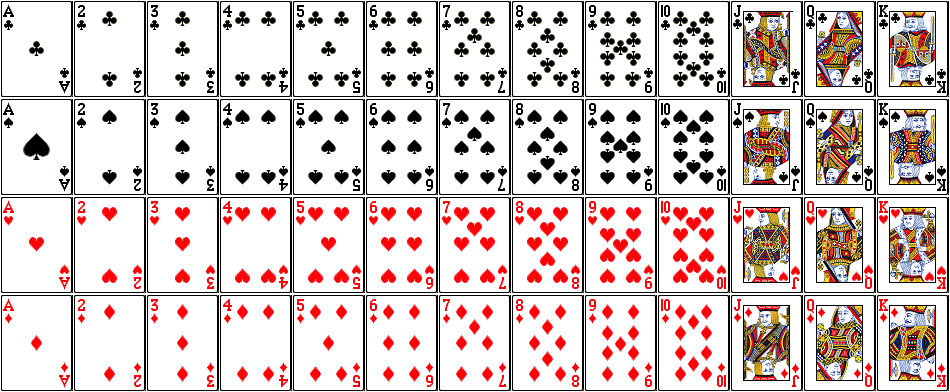
\includegraphics[width=\linewidth]{playing-cards1.png}
\end{center}


\quest{15 min}


\Q Implement the following constructor.
The class has two attributes: \java{rank} and \java{suit}.
Don't think too hard about it.

\begin{javalst}
/**
 * Constructs a face card given its rank and suit.
 *
 * @param rank face value (1 = ace, 11 = jack, 12 = queen, 13 = king)
 * @param suit category ("clubs", "diamonds", "hearts", or "spades")
 */
public Card(int rank, String suit) {
\end{javalst}

\vspace*{-1em}
\begin{answer}
\begin{javaans}
    this.rank = rank;
    this.suit = suit;
\end{javaans}
\end{answer}
\vspace*{-1em}

\begin{javalst}
}
\end{javalst}


\Q In one line of code, declare an array of strings named \java{suits} and initialize its contents to the four possible suits as shown above.

\vspace*{-1ex}
\begin{answer}
\begin{javaans}
    String[] suits = {"clubs", "spades", "hearts", "diamonds"};
\end{javaans}
\end{answer}


\Q Write several lines of code to declare and create an array of 52 \java{Card} objects.
Use nested \java{for} loops to construct \java{Card} objects in the order of the Model.
Make use of your \java{suits} array from the previous question.
Discuss with your team how you will keep track of the array index.

\vspace*{-1ex}
\begin{answer}[11em]
\begin{javaans}
Card[] cards = new Card[52];
int index = 0;
for (String suit : suits) {
    for (int rank = 1; rank <= 13; rank++) {
        cards[index] = new Card(rank, suit);
        index++;
    }
}
\end{javaans}
\end{answer}


\Q Describe what the following code does and how it works. (Note: You've come a long way this semester, to be able to understand this example!)

\begin{javalst}
public static Card[] sort(Card[] deck) {
    if (deck == null) {
        System.err.println("Missing deck!");
        return null;
    }
    Card[] sorted = new Card[deck.length];
    for (Card card : deck) {
        int index = card.position();
        sorted[index] = card;
    }
    return sorted;
}
\end{javalst}

\begin{answer}[5em]
This example sorts an array of cards.
It first validates the arguments, then it creates a new array of cards and assigns each \java{Card} reference according to its known position in the deck.
\end{answer}


\Q Write a static method named \java{inDeck} that takes a \java{Card[]} representing a deck of cards and a \java{Card} object representing a single card, and that returns \java{true} if the card is somewhere in the deck of cards. Be sure to use the equals method of the \java{Card} object to make comparisons.

\vspace{-1ex}
\begin{answer}[11em]
\begin{javaans}
public static boolean inDeck(Card[] deck, Card card) {
    for (Card c : deck) {
        if (c.equals(card)) {
            return true;
        }
    }
    return false;
}
\end{javaans}
\end{answer}
